% !TeX root = surgery.tex
\section{The Printed Editions}

The careful survey of printed editions of the \SS\ by Meulenbeld lists no fewer than 
44 entries.\footcite[IIB, 311--314]{meul-hist}  These range from the first edition 
by 
Madhusūdana Gupta (\citeyear{gupt-1835}) to editions in the 1970s. The 
number of 
reprints and editions since that time might almost double that number.  
Translations begin with Hessler's Latin translation in \citeyear{hess-1855} and 
continue up to the present in scores of publications in many 
languages.\footcites[E.g.,]{zysk-1984}[IIB, 314--315]{meul-hist}

\subsection{The vulgate}


The great ayurvedic scholar Yādavaśarman Trivikrama Ācārya produced three
successive editions of the \SS\ with the commentary of Ḍalhaṇa, in 1915, 1931 and
1938.  These editions, especially the last, are generally considered the most
scholarly and reliable editions of the work, and have been constantly reprinted up
to the present day.\footnote{See also the studies of these editions by
    \textcites[\S 1.2]{kleb-2021b}[143--144]{wuja-2013}.}  We refer to the last of
    these editions as “the vulgate.”

The 1915 edition was based on three manuscripts.  The 1931 edition used another
seven manuscripts plus two printed editions.  For his final 1938 edition, Ācārya
used a further three manuscripts.\footnote{The following account is
paraphrased from \citeauthor{vulgate}'s own account of their sources
\citep[22]{vulgate}.}  These sources are described as follow, with an overview in
Table~\ref{tableofeds}.

\subsection{The sources of the 1915 edition}

\begin{enumerate}
    \item[1] Calcutta, Royal Asiatic Society.  Covers the \emph{sūtra, nidāna, śārīra 
        and 
        kalpa sthāna}s.  
    
    \item [2] Jaipur, Pandit Gaṅgādharabhaṭṭaśarman, lecturer at the Royal 
    Sanskrit University.  Covers the \emph{cikitsāsthāna} and the 
    \emph{uttaratantra}.
    
    \item [3]  Bundi, my great friend the royal physician Paṃ.\ Śrīprasādaśarman  
    Covers the \emph{uttaratantra}.
\end{enumerate}

\subsection{The sources of the 1931 edition}

\begin{enumerate}
    
    \item[1] Vārāṇasī, professor of literature, the great Gaurīnāthapāṭhaka.  With 
    the 
    \emph{Nibandhasaṅgraha}. Covers the \emph{nidānasthāna} and 
    \emph{uttaratantra}.
    
    \item [2]  Ahmedabad.  My friend Sva.\ Vā.\ Vaidya Raṇachoḍalāla 
    Motīlālaśarman.  
    With the \emph{Nibandhasaṅgraha}.  Covers the \emph{śārīrasthāna}.
    
    \item [3] From the personal library of my great friend Sva.\ Vā.\ Vaidya
    Murārajīśarman. Extremely old. No commentary.  Covers the 
    \emph{śārīrasthāna}.
    
    \item [4]  Puṇe, BORI library.  With the \emph{Nibandhasaṅgraha}. Covers the
    \emph{śārīrasthāna}.\footnote{Not one of the three MSS of the
    \emph{śārīrasthāna} described in \cite{shar-vaid}.}
    
    \item [5]  Puṇe, BORI library.  With the \emph{Nibandhasaṅgraha}. Complete.  
    With some damaged folia.
    
    \item [6]  Bombay, Asiatic Society.  Incomplete.\footnote{Possibly 
    \MScite{Mumbai 
    AS B.I.3} or \MScite{Mumbai AS B.D.109} \citep[v.\,1, \# 212 and 
    213]{vela-1930}.  But both these have the \emph{Nibandhasaṅgraha}.  The 
    first 
    covers only the \emph{śārīrasthāna}; the second may be complete, but 
    Velankar calls it 
    only “disorderly.”}
    
    \item [7] Varanasi, the private library of Vaidya Tryambakaśāstrī.  Covers the 
    \emph{cikitsāsthāna}.  The variant readings of this MS were compiled by Prof.\ 
    %    Guruprasādaśāstrī and supplied to Ācārya.
    
    \item [8]  A printed edition together with the commentary 
    \emph{Suśrutasandīpanabhāṣya} by Professor Hārāṇacandra Cakravārtti. 
    Complete work.
    This is the 1910 Calcutta edition numbered “t” by \citet[IB, 
    312]{meul-hist}.\footcite{bhat-1917}
    
    \item [9] A printed edition of the first 43 chapters of the
    \emph{sūtrasthāna}, printed in Bengali script, with the commentaries
    \emph{Bhānumatī}, \emph{Nibandhasaṅgraha}, edited by Vijayaratnasena and
    Niśikāntasena. This is the 1886 Calcutta edition numbered “g” by \citet[IB,
    311]{meul-hist}.\footcite{sena-1886}
    
\end{enumerate}

%
\begin{table}
    \caption{The sources of Yādavaśarman T. 
        Ācārya's 
        three editions:\\ manuscript coverage (\newmoon) and print coverage
        ($\circ$). \label{tableofeds}}
    \vspace{.5\baselineskip}
    
    \begin{tabular}{c|ccc|ccccccccc|ccc}
        \toprule
        %        \multicolumn{16}{c}{\emph{Manuscripts (\newmoon) and print 
        %editions 
        %                ($\circ$)}} \\
        \emph{edition}            &\multicolumn{3}{c}{1915}
        &                \multicolumn{9}{c}{1931} 
        &              \multicolumn{3}{c}{1938} \\
        
        \emph{source}         & 1 & 2 & 3 & 1 &2  &3  &4  &5  &6  &7  &8  &9  &1  
        &2 &3 \\
        
        
        \midrule
        
        \emph{sthāna} &&&&&&&&&&&&&&&\\        
        
        \emph{sū}. &  \newmoon&  &  &
        &  &  &  & \newmoon & ? &  & $\circ$ & 
        $\circ^\dag$ &  
        \newmoon & &\newmoon \\
        
        \emph{ni}. &\newmoon  &  &  &
        \newmoon &  &  &  &  \newmoon&  ?&  & $\circ$ &  &  
        \newmoon&\newmoon & \newmoon\\
        
        \emph{śā}. &  \newmoon&  &  &
        & \newmoon & \newmoon & \newmoon & \newmoon &  ? &  &  
        $\circ$&  &  
        \newmoon& &\newmoon \\
        
        \emph{ci}. &  & \newmoon &  &
        &  &  &  &\newmoon & ? &  \newmoon&$\circ$  &  &
        \newmoon & &\newmoon$^{\dag\dag}$ \\
        
        \emph{ka}.  &\newmoon  &  &  &
        &  &  &  &\newmoon  &  ?&  & $\circ$ &  &  
        \newmoon  & & \\
        
        \emph{utt}.  &  & \newmoon &\newmoon  &
        \newmoon  &  &  &  & \newmoon & ? &  & $\circ$ &  &  
        & & \\
        \bottomrule
    \end{tabular}
\medskip

{\small
$\dag$    Covers chapters 1--43 only. \quad
$^{\dag\dag}$ Covers chapters 1--9 only.
    \par}
\end{table}  
% notes to table 2.
%    \addtocounter{footnote}{-1}
%    \footnotetext{Covers chapters 1--43 only.}
%    \stepcounter{footnote}
%    \footnotetext{Covers chapters 1--9 only.}

%
\subsection{The sources of the 1938 edition}
% \coffeestainC{1}{1}{180}{0}{-5 mm}
\begin{enumerate}
    \item [1]  Gwalior, from the library of my great friend Paṃ.\ Rāmeśvaraśāstrin 
    Śukla. 
    Covers the \emph{sūtra, nidāna, śārīra, cikitsā and kalpasthāna}s.
    
    \item[2] Bikaner, from the library of the Royal Palace, supplied by Paṃ.\ 
    Candraśekharaśāstrin. Contains the commentary 
    \emph{Nyāyacandrikāpañjikāvyākhyā} by Gayadāsa.  Covers the 
    \emph{nidānasthāna}.      
    This is almost certainly \MScite{Bikaner Anup 
        4390}.\footnote{See Dominik Wujastyk, “MS Bīkāner AnupLib 4390.” 
    \emph{Pandit}. 
    <\url{http://panditproject.org/entity/108068/manuscript}>.}
    
    \item [3] Kathmandu, located in the private library of the Royal Guru Hemarāja 
    Śarman.  An extremely old palm-leaf manuscript. Readings from this MS were 
    compiled by Paṃ Nityānandaśarman Jośī and sent to Ācārya. Covers from the 
    beginning of the work to the end of the ninth chapter of the 
    \emph{cikitsāsthāna}.  The 
    siglum for this manuscript in footnotes was \dev{tā} for 
    \dev{tālapatrapustake}. 
\end{enumerate}
\subsection{Evaluation}

Estimates show that there are approximately 230 extant manuscript witnesses for
the \emph{Suśrutasaṃhitā}.\footnote{This figure is arrived at by summing the MSS
    mentioned by \tvolcite{39}[373--375]{ncc} and in the \cite{ngmcp}. The real figure
    could be many scores higher.  Cf.\ the overview at
    \cite{wuja-2020}.\label{SSmss}.}  Although many of these manuscripts cover only
    parts of the whole work, they amount to approximately twenty times the evidence
    that was used by Ācārya for his vulgate editions.

While the descriptions provided by Ācārya of his source materials seems at first
to be moderately comprehensive, Table~\ref{tableofeds} reveals the underlying
paucity of textual sources for these editions.  At first, it appears that fifteen
manuscripts were consulted.  However, we quickly see that two of the sources 
were
other people's printed editions, and one of those covered less than a quarter of
the work (no.\,9 of 1931).  That reduces the manuscript base to 13 manuscripts.
Ācārya does not appear to have seen two of the manuscripts at all, having been
sent collations prepared for him by others (7 of 1931 and 3 of 1938).  Thus,
Ācārya's final edition was based on the personal consultation of eleven partial
manuscripts.   One of them remains unidentified (6 of 1931). Only a single
manuscript covers the whole of the \emph{Suśrutasaṃhitā}, no.\,5 of the 1931
edition.  Manuscript 1 of 1938 is the next most complete, but it omits the
\emph{uttaratantra}, which comprises a third of the work.  Manuscript 1 of the
1915 edition is third in size, but it still omits both of the longest chapters,
and thus offers less than half the work.  For the rest, the evidence is spotty,
with each part of the work being supported by only between four and eight
manuscripts, excluding the printed editions.

Two sources stand out for their historical importance.  The first is no.\,3 of
1931, which Ācārya calls “extremely old.”  It covered the \emph{śārīrasthāna}
only, and unfortunately we know nothing of the later history of this manuscript.
The second is no.\,3 of 1938, which is one of the important Nepalese manuscripts
being considered in the present project. Ācārya's remarks and references to
Hemarājaśarman's introduction to the \emph{Kāśyapasaṃhitā} allow us
to identify this manuscript as \MScite{Kathmandu NAK 
    5-333}.\footnote{\cites[22]{vulgate}[56--57]{hema-1938}. Discussed by
\citet[\S 1.1, 2.3]{kleb-2021b}.  See also \cites[IIB, 
25--41]{meul-hist}[161--169]{wuja-2003}.} The editors of the vulgate, \citeauthor{vulgate}, 
stated that this manuscript covered up to the ninth chapter of the \emph{cikitsāsthāna}, but 
in fact it covers the whole work.\footcite[22]{vulgate}  Perhaps the editors
only received collations for this portion of the manuscript and did not know that it
was a witness for the whole work.

\subsection{The 1939 edition}        
\label{1939edition}

In 1939, Yādavaśarman Trivikrama Ācārya and Nandakiśora Śarman co-edited an
edition of the \emph{sūtrasthāna} of the \emph{Suśrutasaṃhitā} that was 
published
by the Swami Laxmi Ram ayurvedic centre in Jaipur, and printed at the famous
Nirṇayasāgara Press in Mumbai (see 
Fig.\,\ref{bhanumati}).\footnote{\cite{acar-1939}.  The description of 
the sources 
below is based on Yādavaśarman T. Ācārya's  remarks in his introduction 
(pp.\,3--4). See also the remarks on this edition by
\citet[7]{kleb-2021a}.  On the Swami Laxmi Ram
centre, see \cite{hofe-2007}} The text was edited on the basis of the following 
sources.

\begin{figure}[p]
    \centering
    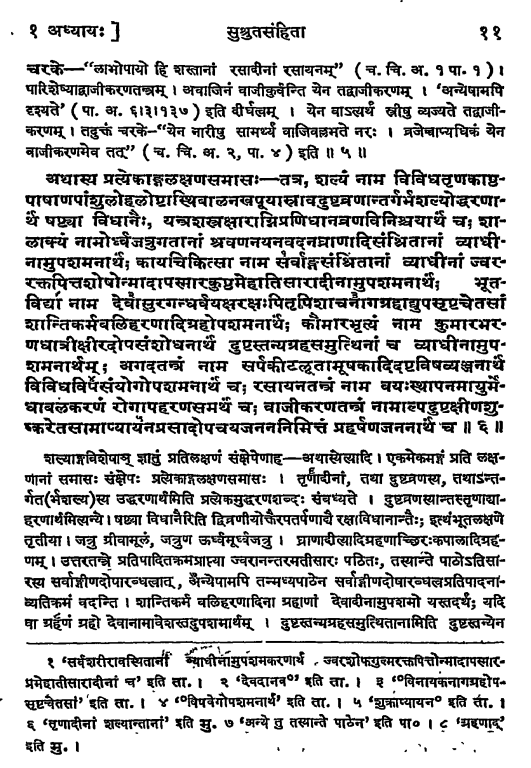
\includegraphics[draft=false,height=.9\textheight]{media/Bhanumati-page-11}
    \caption{A page of the 1939 \emph{Bhānumatī} edition, showing the variant 
        readings in the footnotes.}
    \label{bhanumati}
\end{figure}


\subsubsection{For the Bhānumatī}

\begin{enumerate}
    \item A printed edition.  Covered the \emph{Bhānumatī} up to chapter Su.sū.40.
    The siglum was \dev{mu} for \dev{mudrita}.\footnote{\cite{sena-1886}.  
    The
    manuscript on which this edition was based is probably in the library of the
    Calcutta Sanskrit College, and described in \cite[v.\,X.1]{sast-1917}, which
    is not available to me.  See also \cite[IB, 495, n.\,57]{meul-hist} for
    mention of this manuscript.  The reference at \cite[217]{rao-sans} to CSCL
    accession number 97 in Bengali script may be this manuscript.}
    
    \item A manuscript in the India Office Library library provided through the
    Bhandarkar Oriental Research Institute in Pune.\footnote{At this time,
    manuscripts from Britain were routinely lent to scholars in India and vice
    versa.} This manuscript covered the \emph{Bhānumatī} b up to the end of the
    \emph{sūtrasthāna}.  The siglum was \dev{ha} for
    \dev{hastalikhita}.\footnote{\cite{PP109978}; 
    \MScite{London BL H. T. Colebrooke 908}
    (\href{panditproject.org/entity/109978/manuscript}{PanditProject \#109978},
    consulted on July 03, 2021).}
\end{enumerate}

\subsubsection{For the Suśrutasaṃhitā}

\begin{enumerate}
    \item A palm leaf manuscript from Hemarājaśarman's personal
    library.\footnote{I.e., \MScite{Kathmandu NAK 5-333}.}  The siglum was
    \dev{tā} for \dev{tāḍapatra}.
    
    \item His own published edition. The siglum was \dev{ḍa} for 
    \dev{ḍalhaṇasaṃmataḥ
        pāṭhaḥ}.\footnote{\cite{vulgate}.  It is noteworthy that Ācārya refers to
    his 1938 edition as representing “the Ḍalhaṇa recension.”}
    
    \item Hārāṇacandra Cakravarti's published edition with his own
    commentary.\footcite{bhat-1917} The siglum was \dev{hā}.
\end{enumerate}
%
\subsubsection{Evaluation}

The main innovation of this publication was to present the only surviving part of
the commentary on the \SS\ by the great eleventh-century medical scholar
Cakrapāṇidatta, namely the \emph{Bhānumatī}.\footcite[IA, 374--375 and IB,
495--496]{meul-hist} A secondary purpose was to present the text of the
\emph{sūtrasthāna} as read in \MScite{Kathmandu NAK 5-333}, that had recently 
been
brought to the editors' attention. In their judgement, the Kathmandu manuscript
presented a text that was closer to what Cakrapāṇidatta had before him than the
text according to Ḍalhaṇa.   This was the first \SS\ edition in which Ācārya used
sigla to identify the sources from which variant readings were reported, so while
it has limitations, it for the first time enables us to get some idea of origins
of the text (see Figure~\ref{bhanumati}).

\label{ref:dalhana}Ācārya noted in his introduction that the manuscripts containing  Ḍalhaṇa's
commentary all came together with the root-text of the \SS, and thus the main \SS\
text reflected the readings chosen by Ḍalhaṇa.  But the manuscripts of the
\emph{Bhānumatī} contained the commentary alone, without the root-text, and 
had
many explanations based on different readings of the root-text than those of
Ḍalhaṇa.  In many of these cases it was hard to infer what readings 
Cakrapāṇidatta had before him. But Ācārya noted that Cakrapāṇidatta had a text
before him that had much in common with the text of the Nepalese
manuscript.\footnote{\cite[3--4]{acar-1939}.  See discussion by
\citet[7]{kleb-2021a}.}  

There is compelling evidence that Cakrapāṇidattas's \emph{Bhānumatī} 
commentary
once covered the whole text of the \SS.\footcite[IA, 375]{meul-hist}  The loss of
the rest of the work ranks amongst the greatest disasters in Āyurvedic
literature.  Remarkably, the whole \emph{Bhānumatī} may still have existed in the
early twentieth century. In 1903, Palmyr Cordier reported being privately informed
of a complete copy of the work in a personal manuscript collection in
Benares.\footcite[332]{cord-1903}


\section{The Manuscripts}

Our edition is based on the textual evidence of three manuscripts.  All three were produced 
in the Kathmandu Valley, Nepal and preserved in libraries there. 
\textcites[\S 
2.1]{kleb-2021b} provided a comprehensive description of the individual manuscripts, quotes 
and translates their colophons and thoroughly examines various problems involved in their 
interpretation. That is why we will present only the key data essential for the study of our 
edition in the present paper.
In referring to the manuscripts, we use the sigla K, N and H, which correspond to the initial letters in the names of the libraries and collection where the respective bundles were discovered.

% TODO: \usepackage{graphicx} required
\begin{figure}[t]
    \centering
    \includegraphics[width=1\linewidth]{"media/017r IMG_0065"}
    \caption{Folio 17r of MS Kathmandu Kaiser Library 699.}
    \label{fig:017r-img0065}
\end{figure}


\begin{description}
       
\item[Siglum K (Fig.\,\ref{fig:017r-img0065})] The MS has been preserved at the Kaiser 
Shamsher (KL) library in Kathmandu, accession number KL 699. It was microfilmed and 
catalogued by the NGMPP/ NGMCP as C 80-7.%
    \footnote{%
    See 
    \url{http://catalogue-old.ngmcp.uni-hamburg.de/mediawiki/index.php/C_80-7_Suśrutasaṃhitā}
     (accessed on October 22, 2021).%
    } 
The MS comprises 152 palm-leaf folios that originally belonged to several different codicological units written by different scribes.%
    \footnote{%
    \textcites[46]{bhat-2020} and \textcites[11]{kleb-2021b} agree that four to five scribes were involved in the manuscript's production.
    } 
The folios are 53.5 $\times$ 4.4 cm in size and have two string holes.  The text is written in the so-called transitional Gupta script, with six to eight lines per folio.%
    \footnote{%
    Codicological features of the manuscript, such as the layout, peculiarities of the script, various ornamental and text-dividing symbols and many more, were scrutinized in \textcites{bhat-2020}.
    }
The MS is incomplete and contains a large part of the \emph{Suśrutasaṃhitā} as well as the \emph{Sauśrutanighaṇṭu}.%
    \footnote{%
    See \textcites[11]{kleb-2021b} for a detailed description of the content.%
    }
The date stated in the colophon at the end of the compendium is verified for Sunday, April 13, 
878 \CE. However, some controversy is involved in interpreting the exact roles of two 
persons 
mentioned in the same concluding remarks, someone called Śrī Harṣacandra and Vaidya 
Vasuvarman. \textcites[16]{kleb-2021b} thinks that the former,
\begin{quote}
\ldots either sponsored the copying enterprise or wrote the manuscript himself,
[and that he subsequently]
    donated it to Vaidya Vasuvarman on the condition that he (Vasuvarman)
would study the text and explain it to others. The second condition was that
the manuscript should remain in the family and not be given away either for
sale or as a pawn. If the manuscript sat unused, it should be returned to Śrī
Harṣacandra.\footnote{See \textcites[13--17]{kleb-2021b} for a translation and
    a study of the colophon, as well as an exposition of different positions
    related to its interpretation.}
\end{quote}



% TODO: \usepackage{graphicx} required
\begin{figure}[t]
    \centering
    \includegraphics[width=1\linewidth]{media/A45-05+73274+034cropped}
    \caption{Folios 30r and 30v of MS Kathmandu National Archives 1-1079.}
    \label{fig:a45-0573274044}
\end{figure}

\item[Siglum N (Fig.\,\ref{fig:a45-0573274044})] This MS is kept at the National Archives 
Kathmandu (NAK), under accession number 1-1079 \dev{ka}. It was microfilmed twice by the 
NGMPP as A 45-5(1) and A 1267-11(2).%
    \footnote{%
See 
\url{http://ngmcp.fdm.uni-hamburg.de/mediawiki/index.php/A_45-5_(Suśrutasaṃhitā)}
 (accessed on October 22, 2021)/
    } 
The MS comprises 65 palm-leaf folios, 56 $\times$ 5\,cm in size, with two string holes each, 
and it is bundled together in a composite manuscript with at least one other medical work. 
The text is written in a variety of Newari script, with ca.\ seven lines per folio. Although the 
text contained in the MS does not cover the entire \emph{Suśrutasaṃhitā} and breaks off 
abruptly in the second chapter of the \emph{śārīrasthāna}, the actual MS, as a codicological 
unit, appears complete, that is, no leaf seems to be missing from the originally unitary 
artefact. Based on paleographic considerations, the MS can be dated tentatively to the twelfth 
or thirteenth century.

% TODO: \usepackage{graphicx} required
\begin{figure}[t]
    \centering
    \includegraphics[width=1\linewidth]{"media/dscn2998 fol 022cropped"}
    \caption{Folios 22v and 23r of MS Kathmandu National Archives 5-333.}
    \label{fig:dscn2998-fol-022cropped}
\end{figure}

\goodbreak
\item[Siglum H (Fig.\,\ref{fig:dscn2998-fol-022cropped})] The MS belongs to the historical 
collection of Hemarāja Śarman (fl.\ 
1878--1953) and is currently kept at the NAK under accession number NAK 5-333. It is 
microfilmed twice by the NGMPP as B 29-19 and B 30-15, but the latter microfilm is 
incomplete.%
    \footnote{%
    See 
    \url{http://ngmcp.fdm.uni-hamburg.de/mediawiki/index.php/B_29-19_Suśrutasaṃhitā}
     (accessed on October 22, 2021).
    } 
The manuscript comprises 435 palm-leaf folios,  $34\times5$\,cm in size, with one string-hole 
in the 
middle. It is written in a type of Newari script that is more recent than the one used in N, with 
approximately six lines per folio. The MS is exceptionally well-preserved and complete, 
containing the text of the \emph{Suśrutasaṃhitā} as well as the \emph{Sauśrutanighaṇṭu}. 
The final colophon identifies the scribe of the MS as Vaidya Amarasiṃhaka, son of 
Kamaladatta, and states the date on which he concluded the copying of the text. Both 
reading, that is, deciphering the actual characters, and interpretation of the concerned 
passage involve diverging opinions, all of which concur, however, in assigning the MS to the 
sixteenth century. \textcites[21--26]{kleb-2021b} gives an analytical account of the views 
expressed in literature, considers further options and puts forward his understanding that the 
MS was completed on Sunday, July 29, 1543 \CE.  
\end{description}
  
In future publications, palaeographical features of these 
witnesses will be described.
%\subsection{Features of the manuscript transmission}
% Andrey
%\subsection{Palaeographical features}
%\begin{itemize}
%    \item śrita for śṛta.
%    \item yātri for yātṛ (Su.ka.1.63) % but yātrin is possible
%     \item punarṇṇavā  (Su.ka.1.61) % but an old Nepelase ms. of the Brahmayāmala has 
%%this spelling.
%    \item ś and s in KL 699.
%    \item b and v in KL 699 and NAK 5-333.
%    \item cha and ccha
%    \item line-fillers
%    \item \d n for n (punar\d n\d nav\=a)
%    \item vyājī-kṛ for vājī-kṛ
%\end{itemize}

%\subsection{Chart of characters}
%[[[Put a chart from QuickPalaeographer here.]]]
% We might be able to link to an akṣara table on the website?

\section{Editorial Principles}
\subsection{Method}
The data for the critical edition comes from the witnesses of the Nepalese version, 
which are MS KL 699, NAK 5-333 and NAK 1-1079. Diplomatic transcriptions of 
SS.1.16 of these manuscripts have been created by researchers of the 
\href{https://sushrutaproject.org}{Suśruta 
Project}\space%\footnote{https://sushrutaproject.org, accessed 20/8/2021.} 
according to a subset of TEI Guidelines that has been formulated by Charles 
Li.\footnote{These guidelines are at \url{https://saktumiva.org/wiki/tei}, accessed 
20/10/2021.} MS NAK 5-333 was transcribed first because its script is relatively easy to 
read, the scans are clear, and it is the most complete of the manuscript 
witnesses. Following that, MS KL 699 and MS NAK 1-1079 were transcribed. 

The diplomatic transcriptions were uploaded to Li's manuscript collation platform
Saktumiva, chapter by chapter as they were completed. An electronic edition of the
vulgate of the \SS, that was transcribed, without the commentaries, by Tsutomu
Yamashita and Yasutaka Muroya on the basis of Ācārya's 1931 and 1938 Bombay
editions has also been included in the collation.\footnote{This electronic edition
    is also available on the SARIT website;
    \url{https://sarit.indology.info/susrutasamhita.xml?view=div}, accessed
    20/8/2021. The version at Saktumiva has received several corrections and the intention is 
    to merge these back into the SARIT version eventually.}

Saktumiva's  collation function standardises punctuation and 
orthographic variants according to filters which can be turned off or on. These 
filters enable the editors to ignore \dev{daṇḍa}, numbers and 
\dev{puṣpikā} in the transcripts, as well as orthographic variants, such as 
\dev{ba} and \dev{va}, certain germinated consonants, and \dev{visarga} 
variants. On the basis of the automatic collation, Jason Birch created a provisional 
edition of SS.1.16, which the project's researchers read together at weekly 
seminars. Manuscript images were routinely checked to verify the transcripts, 
particularly when a reading was uncertain; the commentaries of Cakrapāṇidatta 
and Ḍalhaṇa were read, and variant readings reported by these commentators 
were included in notes to the edition. Also, various reference books were 
consulted, such as   \citet{josi-maha,nadk-1954} and \citet{meul-hist}, to 
elucidate the meaning of technical terms and identify relevant information in 
other medical works. 

An initial draft of the translation and many annotations were written by  
Wujastyk during the seminars as the Project researchers discussed the text's 
meaning. The transcripts, provisional edition and translation were uploaded to the 
project's repository at Github on a weekly basis. Therefore, the project's work has 
been publicly available as it evolves. The software tools used in the project have been 
described on the project website.\footnote{\url{http://sushrutaproject.org}, consulted
    15 September 2022.}

%\begin{enumerate}
%    \item
%    \href{https://www.oxygenxml.com.}{oXygen XML editor} (which has plugins for 
%    Github and TEI, and can validate the 
%    code).%\footnote{https://www.oxygenxml.com.}
%    
%    \item
%    \href{http://saktumiva.org.}{Saktumiva} (a platform for producing and 
%    publishing critical editions of Sanskrit texts).%\footnote{http://saktumiva.org.}
%    \item
%    \href{https://tst.hypotheses.org/1738.}{Quick Palaeographer} (a 
%    browser-based tool for reading MS images and developing a catalogue of 
%    character shapes).%\footnote{https://tst.hypotheses.org/1738.}
%    
%    \item
%    \href{https://filezilla-project.org.}{Filezilla} (document transfer to 
%    Saktumiva).%\footnote{https://filezilla-project.org.}       
%    \item
%    \href{https://github.com.}{Github} (document sharing, security and 
%    versioning).%\footnote{https://github.com.}   
%    \item
%    \href{https://www.latex-project.org.}{LaTeX} (document 
%    preparation).%\footnote{https://www.latex-project.org.}  
%    \item
%    \href{https://qdpm.net.}{qdpm} (project 
%    management).%\footnote{https://qdpm.net.}  
%    
%\end{enumerate}

\subsection{Stemma}
The data from transcripts collated by Saktumiva can be exported as a FASTA file 
and aligned according to characters, syllables or words by a program called 
Helayo. The resulting NEXUS file can be read by phylogenetics software to build a 
stemmatic tree.\footnote{This process is discussed in greater detail by Charles Li 
at \url{https://chchch.github.io/sanskrit-alignment/docs/index.html\#tree}, 
accessed 21/8/2021.} This procedure was done with transcripts of several 
chapters of the Nepalese witnesses, and the results confirmed the editors' 
provisional stemmatic hypothesis that 
K and H are more closely related to one another than K and N.\footnote{See 
section `Features of the Manuscript Transmission' for further discussion of this.} 
Given the early date of K and the small number of other surviving witnesses of the 
Nepalese version, the relationship between the manuscripts at our disposal is 
reasonably clear and, in the case of SS.1.16, the manuscript data was largely 
confined to N and H owing to a missing folio of K. Rather than have to assess 
numerous variant readings from a large number of witnesses, the challenge of 
editing has 
been to repair the text where it has become corrupt in the few witnesses available 
to us. 

\subsection{The Edition and Apparatus}

The critical edition of SS.1.16 in this article retains many of the peculiarities of MS 
KL 699 because the editors have endeavoured to present to the reader an 
archetype of the text that was transmitted by this ninth-century manuscript. 
Therefore, the Sanskrit has been standardised as minimally as possible and, 
although the text has been corrected and repaired wherever it was corrupt in the 
witnesses, it has not been normalized or conventionalized to the extent of many 
modern editions of Sanskrit works. 

The editors have assumed that the authors of the Nepalese \SS\ were familiar 
with Pāṇinian Sanskrit and, although there are some non-standard spellings and 
grammatical forms in the text, there are very few instances of 
hyper-Sanskritization, Buddhist-hybrid Sanskrit or Epic forms that would suggest 
that this assumption is unreasonable. Therefore, the editors of SS.1.16 have 
opted to retain some unusual features of the Sanskrit in MS KL 699 when they are 
grammatically correct. For example, in external \emph{sandhi}, the class nasal is 
usually used at the end of a word instead of an \emph{anusvāra} (e.g.,1.16.3, 
\dev{°vācanan dhātry°}), although the \emph{anusvāra} is sometimes used 
(1.16.15, \dev{udakaṃ dhānyāmla°}). In most cases, the consonant following a 
\dev{repha} is doubled, but this is not always the case.\footnote{Examples of 
the germination of consonants are \dev{karṇṇa} (1.16.1 ff), \dev{muhūrtta} 
(1.16.2), \dev{pūrvva} (1.16.2), \dev{gandharvva} (1.16.5), \dev{°mūlair 
mmadhu°} (1.16.5), \dev{vartti} (1.16.6) and \dev{punar vvidhyet} (1.16.6). 
Examples where it does not occur in 1.16 are  \dev{°ārtham} (1.16.8,19), 
\dev{kuryāt} (1.16.16, 32), \dev{°pālir vallūra°} (1.16.10); \dev{°pālir 
vyāyojimaḥ} (1.16.10) and \dev{dīrghaika°} (1.16.10).} Since these 
inconsistencies seem inherent to the transmission of the text and may have even 
been authorial, the critical edition reflects them as they occur in K and, when the 
testimony of K is not available, the witness most similar to K, which is H.


% This is not always consistent: °ārtham (1.16.8,19), kuryāt (1.16.16, 32), °pālir 
%vallūra°  (1.16.10); °pālir vyāyojimaḥ (1.16.10); dīrghaika° (1.16.10).

% external sandhi
% A tendency to favour the use of the class nasal instead of ṃ (e.g.,1.16.3 
%svastivācanan dhātryaṅke), although ṃ is sometimes used (1.16.15 udakaṃ 
%dhānyāmla°)

% germination of consonants after a repha, even between words.
% karṇṇa (1.16.1 ff), muhūrtta (1.16.2), pūrvva (1.16.2), gandharvva (1.16.5), 
%°mūlair mmadhu° (1.16.5), vartti (1.16.6), punar vvidhyet (1.16.6), °pālir 
%nnirvvedhimaḥ
% This is not always consistent: °ārtham (1.16.8,19), kuryāt (1.16.16, 32), °pālir 
%vallūra°  (1.16.10); °pālir vyāyojimaḥ (1.16.10); dīrghaika° (1.16.10).

The Nepalese manuscripts often have an \emph{anusvāra} before a 
\dev{daṇḍa} at the end of a sentence or verse. Whether these 
\emph{anusvāra}s should be changed to the consonant \dev{m} is a moot 
question because there is no Pāṇinian concept of `end-of-sentence' and his rules 
on \emph{sandhi} are contingent on the close contact of  sounds 
(\emph{saṃhitā})\q{refs?}. However, it is reasonable to assume that at the end 
of a verse, paragraph or sentence the speakers would have paused for breath or 
thought, so \emph{sandhi} should be applied, in which case a final 
\emph{anusvāra} or class nasal of the following consonant is changed to 
\dev{m}.  Nonetheless, this remains an assumption about how the text would 
be pronounced. Therefore, in a critical edition, inserting \emph{daṇḍa}s and 
changing \emph{anusvāra}s to \dev{m} before them are subjective decisions 
by the editors. The scribal use of \emph{daṇḍa}s and \emph{anusvāra}s in the 
Nepalese manuscripts can be seen in the digital edition if one switches off the 
filters for ignoring \emph{daṇḍa}s and final \emph{anusvāra} variants. 

Unconventional spellings and grammatical forms have been retained and noted in 
the annotations to the translation. However, the editors have corrected scribal 
errors and repaired corruptions in the transmitted text with conjectures wherever 
possible. Therefore, although the edition retains many of the peculiarities of the 
Nepalese manuscripts, it is not a diplomatic transcript or a hybrid of diplomatic 
and critical editing because the features of the transmitted text have been 
retained or changed deliberately, and the reasons for doing so are given in either 
the introduction or, in more specific cases, the annotations to the translation.

\subsection{Printed Edition}
The editors intend to produce both printed and digital editions of the Nepalese 
\SS. Since the print and digital environments differ markedly, each edition has 
its own format. The printed edition of SS.1.16 in this article has four layers of footnotes. The first layer reports the witnesses that have been collated. Line numbers and lemmata have been used to identify the witnesses that have been collated for a particular section of the text, as seen in the following example.
\begin{quote}
\dev{1–7 athātaḥ – °viddhaliṅgam} ] MSS K, H, and N
\end{quote}
The above entry means that a textual passage beginning with \dev{athātaḥ} on line 1 and ending with \dev{°viddhaliṅgam} on line 7 is attested by manuscripts K, H and N. This layer also indicates passages that are missing or omitted in a particular witness. 

The second layer of footnotes reports the variant readings of the Nepalese witnesses. This apparatus is negative, that is to say, only the testimony of the variant readings have been reported, and not that of the lemma. The following entry is an example of the apparatus' syntax:
\begin{quote}
\dev{5 pratanuṃ ]  pratanū} N H 
\end{quote}
This entry means that on line five of the edition the editors have chosen to read 
\dev{pratanuṃ}\,, instead of \dev{pratanū}\,, which is attested by witnesses N and H. The 
reader can infer that \dev{pratanuṃ} is attested by K because the first layer of footnotes 
indicate that K has been collated here. In prose passages, the lemmata and 
variants consist of corresponding words and, in verses, corresponding syllables. Emendations by the editors are indicated by the abbreviation \emph{em}., and omissions and suppletions in the witnesses are indicated by \emph{om.} and \emph{add}., respectively. A wavy line under a letter means that it is unclear to the editors. If some text has been deleted by a scribe, it is underscored by double lines. 

The third layer of footnotes contains the variant readings of the vulgate, which have been presented in the same format as the second layer. If a reading of the vulgate has been accepted by the editors against different readings in the Nepalese witnesses, the siglum for the vulgate (i.e., A) has been placed next to lemma in the second layer of footnotes. 

Various testimonia and notes have been included in the fourth layer of footnotes. The testimonia mainly consists of the variant readings noted by the commentators Cakrapāṇidatta and Ḍalhaṇa. Those known to Gayadāsa may be added in future publications. The notes include brief comments on certain emendations and editorial decisions. More elaborate discussions on such issues have been included in the annotations to the translation.

\subsection{Digital Edition}
Instructions for reading the digital edition have been provided by  Li at 
\href{https://saktumiva.org/wiki/users}{Saktumiva}. In brief, you can 
generate the apparatus by choosing a base text and one or more of the other 
witnesses. You can also choose to hide or ignore in varying degrees TEI 
tags, punctuation and orthographical variants in the transcripts of the witnesses. 
On the right side of the text, the digital edition displays an apparatus that is 
negative in so far as the lemma and its witnesses are not included. This apparatus 
truncates variants wherever possible. 

\begin{figure}[t]
    \centering
    %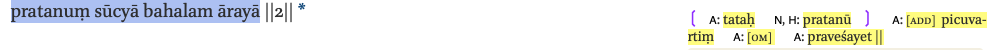
\includegraphics[draft=false, width=\textwidth]{media/SS.1.16.3b}
    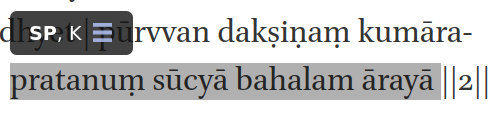
\includegraphics[draft=false,width=.5\textwidth]{media/SS.1.16.3c}
    \quad
    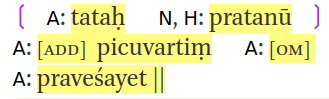
\includegraphics[draft=false,width=.35\textwidth]{media/SS.1.16.3d}
    \caption{The digital edition of SS.1.16.3}
    \label{SS.1.16}
\end{figure}
For example, as seen in Figure~\ref{SS.1.16}, the apparatus for the words 
\emph{pratanuṃ sūcyā bahalam ārayā} is on the right side of the display. 
This entry means that the editors have chosen to read 
\emph{pratanuṃ}, which the reader must infer is attested by K, whereas A has 
\emph{tataḥ} and N and H \emph{pratanū}. Witness A has added the word \emph{picuvartiṃ} after \emph{tataḥ}, omitted \emph{sūcyā bahalam },\footnote{The omitted words are displayed by hovering the cursor over [OM] adjacent to A in the apparatus.} and has \emph{praveśayet} instead of \emph{ārayā}, which is attested by all of the Nepalese witnesses. 

A popup on a dark background, as shown in Figure~\ref{SS.1.16}, displays the
manuscript sigla for the witnesses that support the selected reading.  The positive
apparatus can be expanded by highlighting with the cursor one or more words, and
even entire passages or verses, and clicking on the collapsed menu icon. As seen
in Figure~\ref{SS.1.16.3}, the positive apparatus of \emph{pratanuṃ sūcyā bahalam
    ārayā} appears in a pop-up window in which the lemma and variants are aligned
according to letters, and the variations are highlighted in yellow.

\begin{figure}[t]
    \centering
    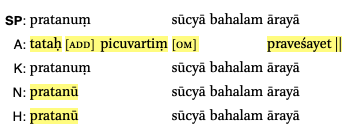
\includegraphics[draft=false,width=.8\textwidth]{media/SS.1.16b.positive}
    \caption{The witnesses to a selected passage of SS.1.16.3}
    \label{SS.1.16.3}
\end{figure}

In both the negative and positive apparatuses of the digital edition, you must
infer conjectures and corrections by the editors. Testimonia and notes are in the
apparatus on the right side of the “provisional edition” text.  They give an
opportunity for the editors to provide scholarly commentary of various kinds, but
the editors cannot write comments directly into the textual apparatus itself,
since it is constructed live each time the text is displayed.





